%% \section{Delta Dictionaries}
\section{Implementation}
\label{sec:DD}

\newcommand{\ddExampleScale}
  %% {0.45}
  {0.50}
  %% {0.55}

\begin{figure}

\centering

%% \begin{figure}[b] %% [H]
\begin{subfigure}[h]{\columnwidth}
  \centering
  \begin{tikzpicture}[nodes = {align = left}]
    \node [scale=\ddExampleScale]
    {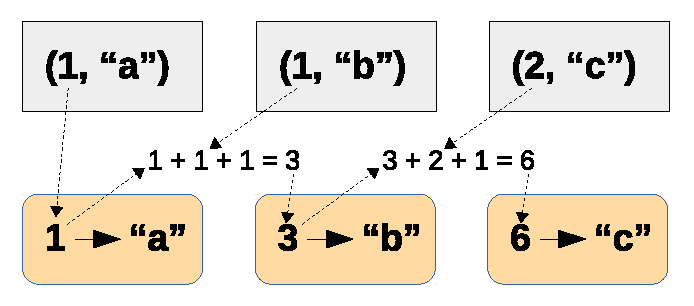
\includegraphics{figs/mech-2-very-short.eps}};
  \end{tikzpicture}
  \caption{An example delta dictionary.}
  %% \caption{What mapping is represented by the \dd~ $\dictP$?}
  \label{fig:dd-example}
\end{subfigure}
%% \end{figure}

\vspace{0.15in}

\begin{figure}[b] %% [H]
  \centering
  \begin{tikzpicture}[nodes = {align = left}]
    \node [scale=.4]
    {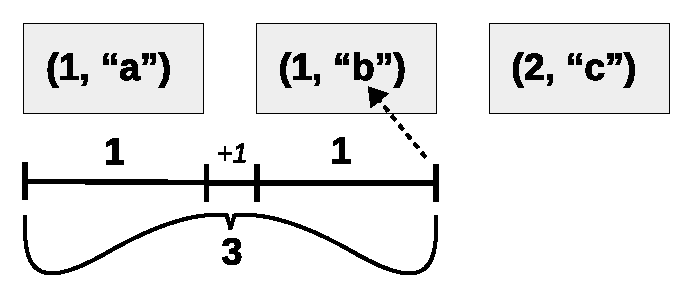
\includegraphics{figs/find-3-very-short.eps}};
  \end{tikzpicture}
  \caption{How do we find key $3$?} %% in the \dd?}
  \label{fig:dd-example-find}
\end{figure}

\vspace{0.15in}

\begin{figure}[H]
  \centering
  \begin{tikzpicture}[nodes = {align = left}]
    \node [scale=.4]
    {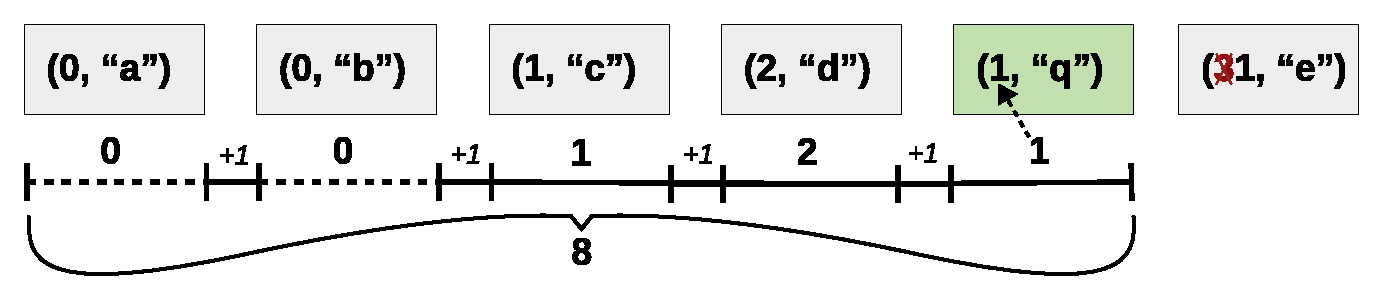
\includegraphics{figs/insert-8.eps}};
  \end{tikzpicture}
  \caption{How do we insert a mapping from key $8$ to value "q"?}
  \label{fig:find-6}
\end{figure}


\caption{Example delta dictionary operations.}
\end{figure}


Our implementation of delta dictionaries and corresponding proofs are formalized in Agda and available in the anonymous supplementary materials.
%
\rkc{But maybe we show Haskell code (rather than Agda) for clarity in explaining the algorithms but their proofs.}

%% \subsection{Delta Indexing}
%% \subsection{Key Types and Deltas}
\subsection{Deltas and Key Types}

Borrowing from association lists, \dds{} use a list-of-pairs, where the first item in each list represents a key and the second is the literal value that is mapped to the represented key.
%
Unlike association lists, the natural number that represents the key is not its literal value.

In order to maintain canonical order, while ensuring that every natural number is valid as the first item in a pair, that number must represent the non-negative difference between the key it represents and the previous key.
%
We call this number a \emph{delta}, alluding to the \emph{delta encoding} technique more commonly harnessed for performance optimization~\citep{XXX}.
%
As described so far, a $0$ offset would correspond to a duplicate key.
%
To prevent duplicate keys from being represented, a delta is actually the offset minus $1$: a delta of $0$ indicates an offset (from the previous key) of $1$, a delta of $2$ indicates an offset of $3$, and so on.
%
The head of the list, however, does not follow the "minus $1$" rule: so the first ``delta'' is interpreted literally, \ie{}~it represents the key value exactly.

\autoref{fig:dd-example} depicts the delta dictionary corresponding to the example from \autoref{sec:Introduction}.

%% \subsection{Bijections to the naturals}
%% \label{sec:DD:bij}
\parahead{Bijections to Natural Numbers}

\rkc{TODO}

Note that the above definitions are in terms of a seemingly arbitrary key type,
and use a function \texttt{convert} to convert terms of that type into naturals.
In Agda, our \dd~ module accepts two parameters - the first is the key type \texttt{Key},
and the second is a type-class \texttt{bij}, whose three members are a \texttt{convert}
function that takes \texttt{Key}s to naturals, and proofs that \texttt{convert} is
injective and surjective. Thus, any key type can be used, as long as the developer
can define a function that converts it to a natural, and prove that that function is
bijective. As an example, we define a \texttt{bij} instance for integers. Other common
key types, such as other numeric types or strings, should be reasonably straightforward
to support. TODO further discussion about how this might be onerous for other key types,
like trees or ADTs. TODO discussion about how this won't work for finite types, like
characters, because we need a true bijection.

Although most types that are suitable for use as keys in the first place can be bijected to the
naturals, for some types defining this bijection may be too awkward or cumbersome, in which case \dds~ may
be a poor choice.

\subsection{Lookup and Insertion}
\label{sec:DD:basics}

\begin{figure*}
%% TODO using alltt temporarily, to inline DD.hs directly
\begin{alltt}
\input{code/DD.hs}
\end{alltt}
\caption{Delta dictionary implementation in Haskell.}
\label{fig:haskell}
\end{figure*}


\autoref{fig:dd-example-find} and \autoref{fig:dd-example-insert} illustrate example \texttt{lookup} and \texttt{insert} operations.
%
These proceed largely as they would for association lists, but working indirectly with keys encoded as natural numbers and, furthermore, differences between these numbers.

\autoref{fig:haskell} presents concrete implementations for \texttt{lookup} and \texttt{insert} in Haskell (rather than Agda) for clarity of presentation.
%
%Having to treat the first delta differently than the rest (literally rather than relatively) is the source of the somewhat technical---through simple---details.

First, we define a helper function \verb+delta+ which computes the delta, \ie{} the offset minus $1$, between two numbers (assuming the second is larger).

Given that, \verb+lookup+ is straightfoward. The \verb+insert+ function is also fairly straightforward - if the first pair is an exact match, then we simply
%
replace the old value with the new one. If the delta to insert is less than delta of the first pair, then we place the delta to insert as the first pair of the new list, and
%
the original first pair will be the second pair of the new list, but using the delta between its original value and the inserted delta.

\nick{The core theorems for lookup and insertion are as follows:}

\subsection{Destruction}

\rkc{move a bunch of that material from Case Study to here}

\rkc{mainly discuss the implementation here. then discuss the difficulties with the library function's type in the properties section below.}

\subsection{Additional Operations}

\rkc{
Our Agda mechanization also defines key deletion, union, map, and to/from-list operations, along
with appropriate metatheory (not reproduced here).
}



%% \subsection{Core properties}
%% \section{Properties}
\subsection{Properties}
\label{sec:DD:props}

%% \subsection{Design Goals}
\parahead{Design Goals}

The \SemInj~ and \EqDec~ theorems, a destruction theorem, and analogs to \emph{contraction} and
\emph{exchange} are defined below, and proven in Agda. \SemTot~ cannot be formally defined - rather
its truth is apparent from the fact that the other theorems do not require their \dd~ arguments to
be refined with validity premises.

\begin{proposition}[\SemTot]

\breakAndIndent
%
\rkc{Blah}

\end{proposition}

\begin{theorem}[\SemInj]
\label{thm:SemInj}

\breakAndIndent
%
For any \dds~ $D_1$ and $D_2$,
%
if for all $k$, $D_1[k] = D_2[k]$,
%
then $D_1 = D_2$.

\end{theorem}

\begin{theorem}[\EqDec]
\label{thm:EqDec}

\breakAndIndent
%
For any \dds~ $D_1$ and $D_2$ whose values are of type $V$,
%
given a function that decides equality for type $V$,
%

\justIndent
%
we can decide that either $D_1 = D_2$ or $D_1 \ne D_2$.

\end{theorem}

%% \begin{theorem}[\EzDstr]
\begin{theorem}[Not-So-Easy Destructibility]
\label{thm:EzDstr}

\breakAndIndent
%
For any \dd~ $D$,

\justIndent \quad
%
either $D = \emptyset$ OR

\justIndent \quad
%
there exist $D'$, $k \notin D'$, and $v$
%
s.t. $D = D' , (k, v)$.

\end{theorem}

%% \subsection{Contraction and Exchange}
\parahead{Contraction and Exchange}

\rkc{Two common properties for PL metatheory.}

\begin{theorem}[Dictionary Contraction]
\label{thm:cont-dicts}

\breakAndIndent
%
For any {\dd}~ $D$,
%
$D, (k, v'), (k, v) = D, (k, v)$.

\end{theorem}

\begin{theorem}[Dictionary Exchange]
\label{thm:exch-dicts}

\breakAndIndent
%
For any {\dd}~ $D$,
%
if $k_1 \ne k_2$, then
%
$D, (k_1, v_1), (k_2, v_2) = D, (k_2, v_2), (k_1, v_1)$.

\end{theorem}
